\documentclass[12pt, a4paper]{article}

\usepackage{mypreamble}
\usepackage{standalone}

\usepackage{tikz}

\usepackage{pdflscape}

\title{Discrete Math II, HW I}
\date{March, 2023}
\author{Aminev Timur, M3104}


\newcommand\EGraph{\mathcal{G}^{*}}
\newcommand\EGraphL{\mathcal{G}}

\begin{document}
\maketitle

\problem The graph of Europe \(\EGraph = \Pair{V, E}\). Let \(\EGraphL\) be the
largest connected component of \(\EGraph\)

\begin{enumerate}[label=\alph*)]
\item \Cref{fig:map_basic} represents \(\EGraph\) with \textbf{no} intersecting
edges
\item \(|V| = 49\), \(|E| = 92\)

In order to count degree of each node, we should go through all edges, and
increment degree of a vertex if the edge contains the vertex. %TODO: link to code
\begin{align*}
\delta(\EGraphL) &= 1 \\
\Delta(\EGraphL) &= 9
\end{align*}

Radius, diameter and center can be obtained by calculating eccentricity for
each vertex (using BFS)

\begin{align*}
\rad(\EGraphL) &= 5 \\
\diam(\EGraphL) &= 8 \\
\mycenter(\EGraphL) &= \{\texttt{RUS}, \texttt{BLR}, \texttt{LTU}, \texttt{POL}, \texttt{UKR}, \texttt{CZE}, \texttt{DEU}, \texttt{SVK}, \texttt{HUN}, \texttt{HRV}, \texttt{AUT}, \texttt{CHE}, \texttt{SVN}\}
\end{align*}

\texttt{Girth} equals 3 --- \(\{\texttt{CHE}, \texttt{AUT}, \texttt{LIE}\}\)

Vertex and edges connectivity are obtained from the following observation:
\texttt{DNK} is conneced only with \texttt{DEU}, therefore
\[\varkappa(\EGraphL) = \lambda(\EGraphL) = 1\]

\item \textbf{Minimum vertex coloring}. Due to \textit{four color theorem},
there're at most 4 colors needed. Let's explore is it possible to use less
colors? Let's try to use 3 colors. However, it's impossible to color countries
\texttt{HRV}, \texttt{SRB}, \texttt{BIH}, \texttt{MNE}. They're all connected
with each other, so three colors is not enough, therefore we have to use four
colors. I used SMT solver (Z3) to find function \(V \to \mathbb{N}\). Here's
\href{https://github.com/ablearthy-itmo-39828cf299f04949c86/discrete-math-2-hw-1/blob/753891b/auto/vertex_coloring.py}{the
script}. See \cref{fig:vertex_coloring_map}.

\item \textbf{Minimum edge coloring}. I used SMT solver (Z3). Here's
\href{https://github.com/ablearthy-itmo-39828cf299f04949c86/discrete-math-2-hw-1/blob/8bc76f0/auto/edge_coloring.py}{the
solver}.
\textit{9} colors is enough. Coloring is shown in \cref{fig:edge_coloring_map}.

\item \textbf{Find the maximum clique}. I wrote the script to find maximum
clique
\href{https://github.com/ablearthy-itmo-39828cf299f04949c86/discrete-math-2-hw-1/blob/1c391015b3b3a8822ac5e7c6f949004ca919e267/auto/find_clique.py}{\texttt{find\_clique.py}}

The maximum clique is of size 4.
\(\texttt{HRV}, \texttt{SRB}, \texttt{BIH}, \texttt{MNE}\)

\item \textbf{Find the maximum stable set}. \href{https://github.com/ablearthy-itmo-39828cf299f04949c86/discrete-math-2-hw-1/blob/79a6584/auto/stable_set.py}{The script}.
\[|S| = 19\]
Countries included in stable set are shown in \cref{fig:stable_set_map}.

\item \textbf{Find the maximum matching}.
\href{https://github.com/ablearthy-itmo-39828cf299f04949c86/discrete-math-2-hw-1/blob/1fae45a/auto/matching.py}{The
script}.
\[|M| = 20\]
Countries included in stable set are shown in \cref{fig:matching_map}.

\item \textbf{Find the minimum vertex cover}.
\href{https://github.com/ablearthy-itmo-39828cf299f04949c86/discrete-math-2-hw-1/blob/cb98748/auto/vertex_cover.py}{The
script}.
\[|R| = 25\]
Countries included in vertex cover are shown in \cref{fig:vertex_cover_map}.

\item \textbf{Find the minimum edge cover}.
\href{https://github.com/ablearthy-itmo-39828cf299f04949c86/discrete-math-2-hw-1/blob/90b7019/auto/edge_cover.py}{The
script}.
\[|F| = 24\]
Edges included in edge cover are shown in \cref{fig:edge_cover_map}.

\item \textbf{Find the shortest closed walk \(W\) that visits every vertex of
\(\EGraphL\)}.

The shorted closed walk is at least of length \(|V| = 44\).
Since there's only one way from \texttt{ESP} to \texttt{ESP}, then in the closed walk
we should visit \texttt{ESP} at least twice. The same goes for \texttt{DEU}.
Therefore, the walk length is at least 46.
In addition to it, we should visit \texttt{FRA} at least three times (that's because
the walk should contain \texttt{MCO} and \texttt{PRT}).
Therefore, the walk length is at least 48.
We should visit \texttt{ITA} at least three times too, because it's connected with \texttt{SMR} and \texttt{VAT}.
Therefore, the walk length is at least 50.
We should visit \texttt{RUS} at least twice, because it's a cut vertex.
Therefore, the walk length is at least 51.

Let's use \textit{\textrussian{метод пристального взгляда}}.
In fact, there's a closed walk of length 51. Therefore, \(|W| = 51\).

\texttt{PRT}--\texttt{ESP}--\texttt{FRA}--\texttt{LUX}--\texttt{BEL}--\texttt{NLD}--\texttt{DEU}--\texttt{DNK}--\texttt{DEU}--\texttt{CZE}--\texttt{POL}--\texttt{SVK}--\texttt{HUN}--\texttt{ROU}--\texttt{MDA}--\texttt{UKR}--\texttt{BLR}--\texttt{LTU}--\texttt{LVA}--\texttt{EST}--\texttt{RUS}--\texttt{NOR}--\texttt{SWE}--\texttt{FIN}--\texttt{RUS}--\texttt{GEO}--\texttt{ARM}--\texttt{TUR}--\texttt{BGR}--\texttt{MKD}--\texttt{GRC}--\texttt{ALB}--\texttt{MNE}--\texttt{ROK}--\texttt{SRB}--\texttt{BIH}--\texttt{HRV}--\texttt{SVN}--\texttt{AUT}--\texttt{LIE}--\texttt{CHE}--\texttt{ITA}--\texttt{SMR}--\texttt{ITA}--\texttt{VAT}--\texttt{ITA}--\texttt{FRA}--\texttt{MCO}--\texttt{FRA}--\texttt{AND}--\texttt{ESP}--\texttt{PRT}

Validness of the closed walk can be checked by \href{https://github.com/ablearthy-itmo-39828cf299f04949c86/discrete-math-2-hw-1/blob/2be1a5d/auto/validate_closed_walk.py}{the script}.
Raw data can be obtained from \href{https://github.com/ablearthy-itmo-39828cf299f04949c86/discrete-math-2-hw-1/blob/fc8406d/data/vertex_closed_walk.txt}{here}.

\item \textbf{Find the shortest closed walk \(U\) that visits every edge of
\(\EGraphL\)}.
%TODO

\item \textbf{Find all biconnected components (blocks) and draw the block-cut tree of \(\EGraph\)}.
To find cut-vertices and blocks we can use algorithm that uses DFS and stores
information about time when a vertex was entered. While searching cut-vertices,
the algorithm also remembers blocks.

Since \(\EGraph\) has more than one connected component, the block-cut tree is
actually \textit{block-cut forest}. Therefore, I'm going to draw the block-cut
tree of \(\EGraphL\) (other components are not fascinating). The raw data can be
found
\href{https://github.com/ablearthy-itmo-39828cf299f04949c86/discrete-math-2-hw-1/blob/6363b0f/data/biconnected_components.txt}{here}.
This was found by
\href{https://github.com/ablearthy-itmo-39828cf299f04949c86/discrete-math-2-hw-1/blob/c81b421/auto/biconnected_components.py}{a script}.

\begin{figure}
\centering
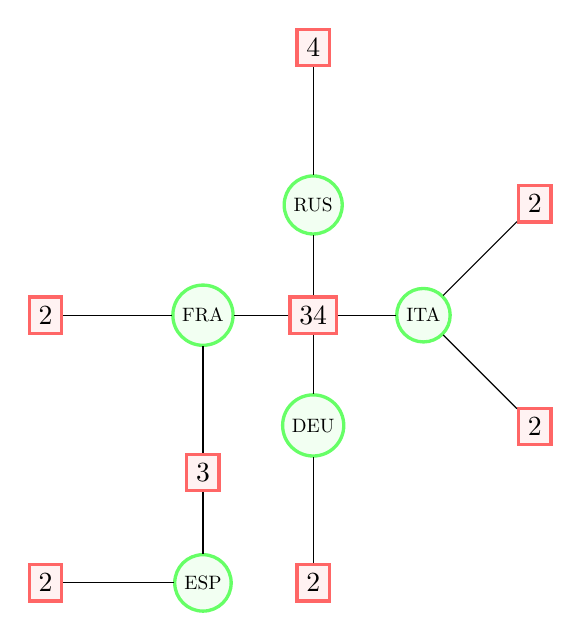
\begin{tikzpicture}[
node distance={20mm},
cutnode/.style={circle, draw=green!60,fill=green!5, very thick, scale=0.7},
blocknode/.style={rectangle, draw=red!60, fill=red!5, very thick}
]
\node[blocknode] (1) {34};
\node[cutnode] (RUS) [above of=1] {RUS};
\node[blocknode] (2) [above of=RUS] {4};
\node[cutnode] (ITA) [right of=1] {ITA};
\node[blocknode] (3) [above right of=ITA] {2};
\node[blocknode] (4) [below right of=ITA] {2};
\node[cutnode] (DEU) [below of=1] {DEU};
\node[blocknode] (5) [below of=DEU] {2};
\node[cutnode] (FRA) [left of=1] {FRA};
\node[blocknode] (6) [below of=FRA] {3};
\node[cutnode] (ESP) [below of=6] {ESP};
\node[blocknode] (7) [left of=ESP] {2};
\node[blocknode] (8) [left of=FRA] {2};

\draw (1) -- (RUS);
\draw (RUS) -- (2);

\draw (1) -- (ITA);
\draw (3) -- (ITA);
\draw (4) -- (ITA);

\draw (1) -- (DEU);
\draw (5) -- (DEU);

\draw (1) -- (FRA);
\draw (6) -- (FRA);
\draw (8) -- (FRA);

\draw (6) -- (ESP);
\draw (7) -- (ESP);
\end{tikzpicture}
\caption{Block-cut tree}\label{fig:block-cut-tree}
\end{figure}

The block-cut tree is shown in \cref{fig:block-cut-tree}.

\end{enumerate}



\begin{landscape}
\begin{figure}
\centering
\includestandalone[mode=build,width=0.95\linewidth]{maps/basic}
\caption{Basic map}\label{fig:map_basic}
\end{figure}
\end{landscape}

\begin{landscape}
\begin{figure}
\centering
\includestandalone[mode=build,width=0.95\linewidth]{maps/vertex_coloring}
\caption{Vertex coloring}\label{fig:vertex_coloring_map}
\end{figure}
\end{landscape}

\begin{landscape}
\begin{figure}
\centering
\includestandalone[mode=build,width=0.95\linewidth]{maps/edge_coloring}
\caption{Edge coloring}\label{fig:edge_coloring_map}
\end{figure}
\end{landscape}

\begin{landscape}
\begin{figure}
\centering
\includestandalone[mode=build,width=0.95\linewidth]{maps/stable_set}
\caption{Maximum stable set}\label{fig:stable_set_map}
\end{figure}
\end{landscape}

\begin{landscape}
\begin{figure}
\centering
\includestandalone[mode=build,width=0.95\linewidth]{maps/matching}
\caption{Maximum matching}\label{fig:matching_map}
\end{figure}
\end{landscape}

\begin{landscape}
\begin{figure}
\centering
\includestandalone[mode=build,width=0.95\linewidth]{maps/vertex_cover}
\caption{Minimum vertex cover}\label{fig:vertex_cover_map}
\end{figure}
\end{landscape}

\begin{landscape}
\begin{figure}
\centering
\includestandalone[mode=build,width=0.95\linewidth]{maps/edge_cover}
\caption{Minimum edge cover}\label{fig:edge_cover_map}
\end{figure}
\end{landscape}
\end{document}
